%%% WhitePaper.tex ---

%% Author: Yi Cao
%% Version: $Id: WhitePaper.tex,v 0.0 2017/01/26 17:11:55 ycao

%% revision: WhitePaper.tex,v 0.0 2017/01/26 17:11:55 ycao

%%%---------------------------------------------------------------------

\documentclass[11pt]{article}
\usepackage[letterpaper, portrait, top=1in, bottom=1in, left=1in, right=1in]{geometry}
\usepackage{fancyhdr}
\usepackage{lastpage}
\usepackage{graphicx}
\pagestyle{fancy}
\lhead{\textbf{ZTF White Paper}}
\rhead{\textbf{}}
\cfoot{\thepage/\pageref{LastPage}}
\usepackage{multicol}
\usepackage{natbib}
\usepackage[font=small, labelfont=bf]{caption}
\usepackage{wrapfig}
\usepackage[shortlabels]{enumitem}
\usepackage{amssymb}
\usepackage{amsmath}
\setlength{\multicolsep}{2.0pt plus 2.0pt minus 1.5pt}
\usepackage{url}


% journals
\newcommand\apj{ApJ}
\newcommand\nat{Nature}


\begin{document}

%%%%##########################################################################

\begin{center}
  \textbf{\Large Young Type Ia Supernova Science In ZTF}\\
  Last Update: \today
\end{center}


\section{Scientific Motivation}
\label{sec:scientific_motivation}

Despite the facts that thousands of Type Ia supernovae (SNe Ia) have
been discovered and that a large number of high-quality light curves
and spectra have been obtained, The origin of SNe Ia and their
explosion mechanism remain mysterious. Recent developments in theory
and observation, has shown that systematical observations of
extraordinarily young SNe Ia is a promising avenue to make big
progresses in this field.

Specifically, ZTF with its huge field of view, has great potentials in
investigating the following three issues of SNe Ia: (1) estimating the
fraction of SNe Ia born in the single degenerate channel with the
SN-companion collision signatures; (2) investigating the initial rise
behavior and its connection to $^{56}$Ni mixing in the ejecta; (3)
characterizing SN-CSM interaction to probe the mass loss history of
the progenitor system.

\subsection{SN-Companion Collision}
\label{sec:sn_companion_collision}

The single degenerate (SD) and double degenerate (DD) channels are two
main scenarios for progenitors of SNe Ia. SN-companion collision are
only expected from the SD channel and thus the emission from
SN-companion collision serve as a ``smoking gun'' for the SD channel.

According to the model in \citet{2010ApJ...708.1025K}, the collision
emits an X-ray flash on timescales of $\sim 10\,\textrm{mins}$ and
then heats up surrounding ejecta material into high temperatures. Then
the hot ejecta material produces thermal emission with a spectrum that
peaks in the UV. Using the analytical equations in
\citet{2010ApJ...708.1025K} and the approximation of angular
dependence in \citet{2012ApJ...749...18B}, and assuming a typical
binary separation $a=10^{13}\,\textrm{cm}$, an ejecta mass
$M=1.4M_\odot$, and a constant opacity
$\kappa=0.2\,\textrm{cm}^2\,\textrm{g}^{-1}$, we calculate the
expected thermal emission from the SN-companion collision as viewed in
different angles and in the UV and optical bands (Figure
\ref{fig:sn_companion_collision}).

\begin{figure}[htb]
  \centering
  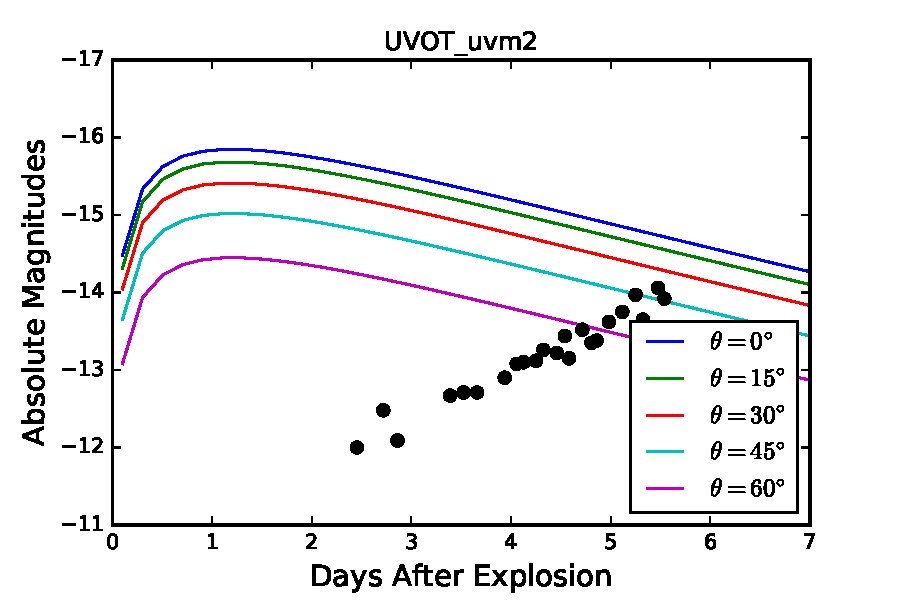
\includegraphics[width=0.475\textwidth]{UVOT_uvm2.pdf}
  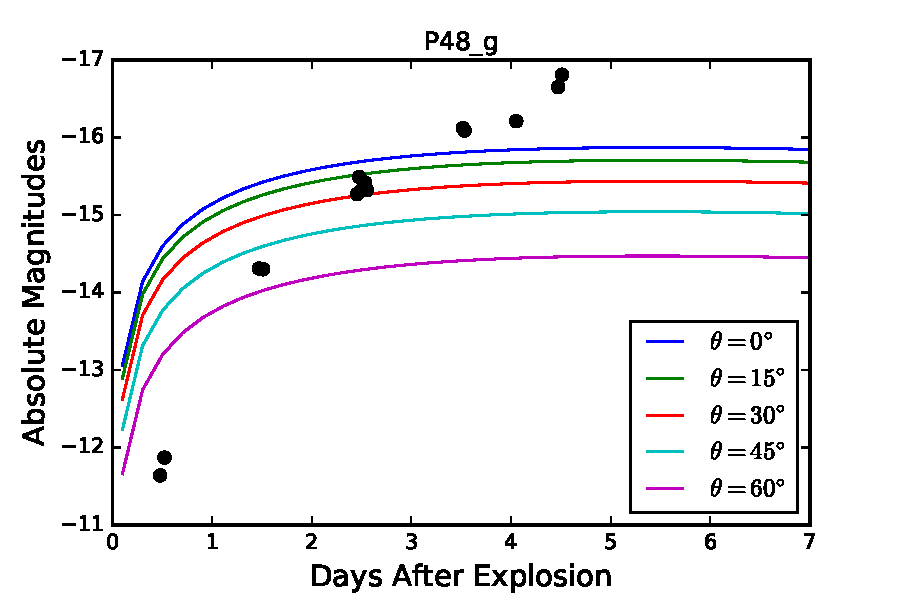
\includegraphics[width=0.475\textwidth]{P48_g.pdf}  
  \caption{Theoretical light curves of SN-companion collision in a
    binary separated by $10^{13}\,\textrm{cm}$ in the UVOT
    \textit{uvm2} (left panel) and PTF \textit{g} (right panel)
    bands. The ejecta mass is assumed to be $1.4M_\odot$, and the
    opacity of the ejecta is
    $0.2\,\textrm{cm}^{2}\,\textrm{g}^{-1}$. Colors are used to
    represent different viewing angles. In comparison, the observed
    light curve of SN2011fe is shown in black circles.}
  \label{fig:sn_companion_collision}
\end{figure}

Figure \ref{fig:sn_companion_collision} clearly shows that the UV
wavelengths are much more preferred for three reasons than the optical
in searches for SN-companion collision signatures.  First, due to the
high temperatures ($\gtrsim10^{4}\,\textrm{K}$) of the emitting
region, the SN-companion collision is brighter in the UV. Second, the
contrast between the SN-companion collision signature and the SN
emission is much larger in the UV than in the optical. Third, since
the SN-companion collision produces a peak in the UV, it is easier to
decouple different light curve components. Therefore, given the
currently available instruments in the optical and UV, the best
strategy to search for the SN-companion collision signature is to
discover SNe in a wide-field experiment of one-day cadence and trigger
space-based UV follow-up observations (e.g., \textit{Swift}/UVOT)
within a day of discovery.

\subsection{Diversity Of Radioactively Powered Light Curves}
\label{sec:diversity_of_radioactively_powered_light_curves}

Thanks to the almost constant mass of ejecta and synthesized
$^{56}$Ni, the light curves of SNe Ia around peak are quite
uniform. However, their early-phase light curves may show great
diversity. Since different mechanisms or stochastic procedures in the
SN explosion may lead to distinct degrees of mixing in the ejecta, the
moment when the first photons from the radioactive decay escape the SN
ejecta is characterized by the photon diffusive timescale from the
shallowest layer with deposited $^{56}$Ni to the photosphere of the
ejecta. For the same reason, the initial rise rate also depends on the
shallowest distribution of $^{56}$Ni.

\citet{2016ApJ...826...96P} calculated the early light curve of SNe Ia
with weak and strong mixing (left panel of Figure
\ref{fig:early_light_curve}) and found that (1) a SN with deeply
deposited $^{56}$Ni has a dark period of up to $\simeq$ two days
before the rise of its radioactively powered light curve, while a SN
with strong mixing has a negligible dark period; (2) the initial rise
rate of a SN with weak mixing is less than that of a SN with strong
mixing.  Hence, characterizing the initial rise rates of SNe Ia will
allows us to probe the mixing degrees of $^{56}$Ni in the ejecta, which
in turn constrains the explosion mechanism. According to the left panel
of Figure \ref{fig:early_light_curve}, a one-day cadence survey in the
optical is sufficient to carry out this study.

\begin{figure}[htb]
  \centering
  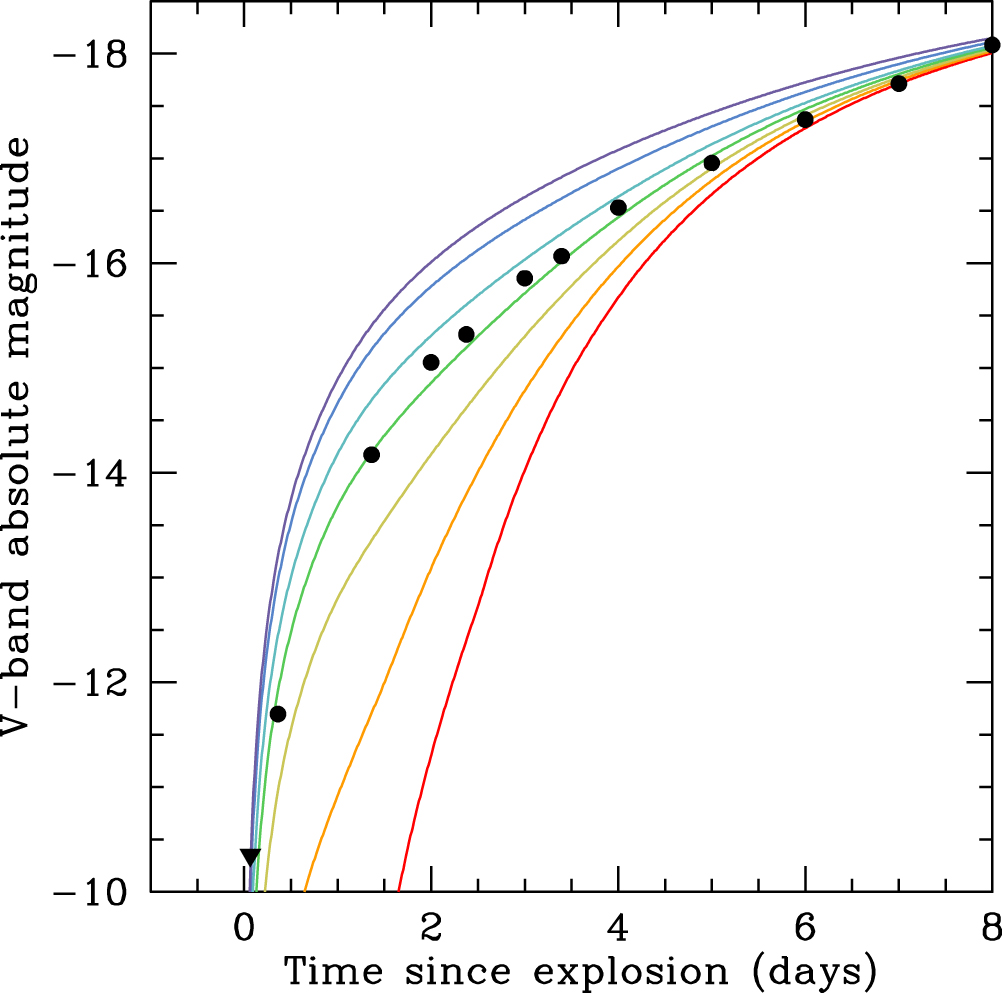
\includegraphics[width=0.475\textwidth]{deposition.jpg}
  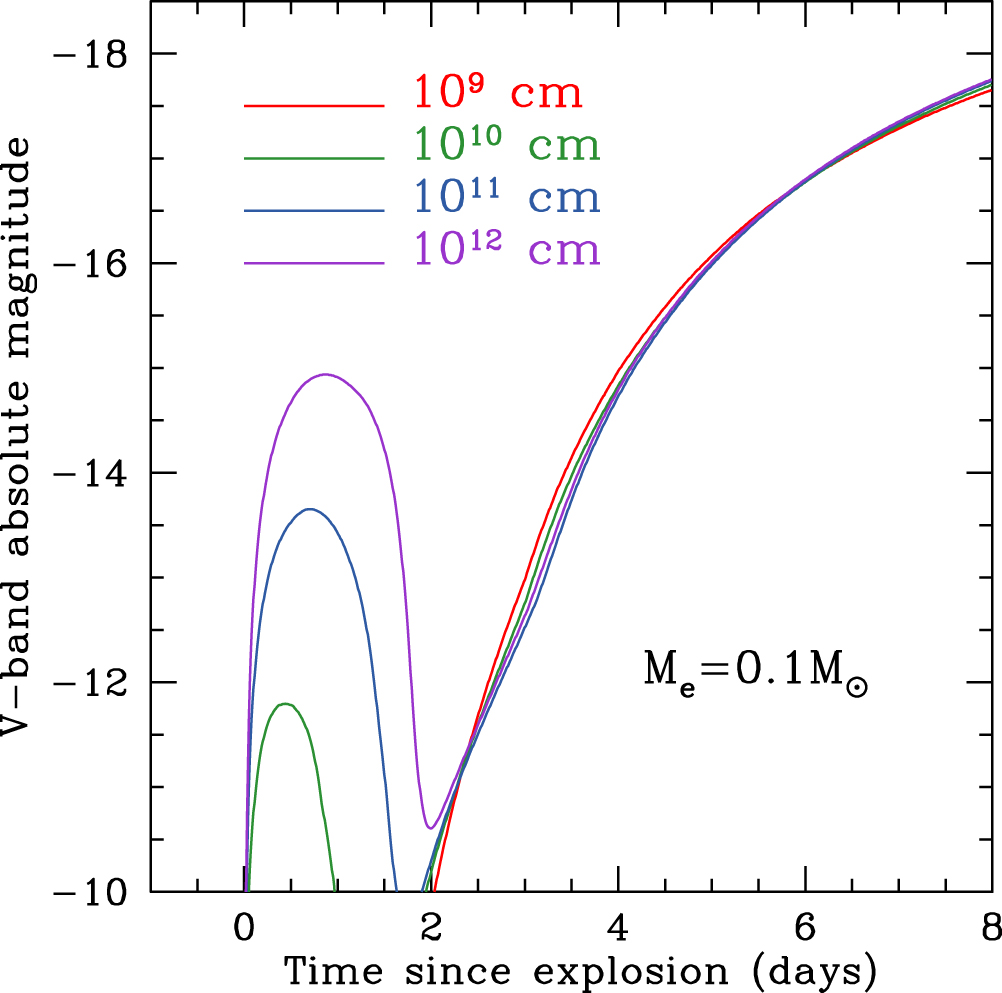
\includegraphics[width=0.475\textwidth]{extended_material.jpg}
  \caption{
    \textit{Left panel:}
    The radioactively powered light curves of SNe with weak
    (red) and strong (blue) mixing. The circles and triangle are the
    observed light curve of SN2011fe. [Figure 7 in
    \citet{2016ApJ...826...96P}]
    \textit{Right panel:}
    The early light curve peak produced by an extended material of
    $0.1M_\odot$ at different distances from the explosion center.
    The SN ejecta is assumed to have weak mixing of $^{56}$Ni .
    [Figure 10 in \citet{2016ApJ...826...96P}]
  }
  \label{fig:early_light_curve}
\end{figure}

\subsection{SN-CSM Interaction}
\label{sec:sn_csm_interaction}

Most progenitor scenarios of SNe Ia involve some sort of mass transfer
process, which in principle should leave excess material around the
progenitor system.  Should this circumstellar medium (CSM) exists at
the time of SN explosion, the ejected material will interact with the
CSM, imprinting observable signatures in the early emission of the SN.

\citet{2016ApJ...826...96P} discussed the possible signature from the
SN-CSM interaction. After being heated up by the SN shock, the CSM
will emit thermal radiation as it cools down. According to
calculations, the SN-CSM collision will produce a light curve peak at
early phases (right panel of Figure
\ref{fig:early_light_curve}). Should SN-CSM interaction exists, this
extra peak in the early-phase SN Ia light curve can be captured by a
one-day cadence survey.


\section{Proposed experiments}
\label{sec:proposed_experiments}

To meet the scientific goals listed above, we request the following
experiment:
\begin{itemize}
\item \underline{Pointings}: Given the simulated light curves and the
  sensitivity of ZTF, the early-phase light curve is only detectable
  for SNe within 100\,Mpc.  Hence the pointings should be focused on
  local structures within this distance.
\item \underline{Cadence}: According to the simulated light curves, a
  one-day cadence is needed. In order to remove moving objects, every
  pointings should be visited twice each night.
\item \underline{Filter}: Given the fact that the expected light
  curves of SN-companion collision are brighter in the \textit{g} band
  and the fact that the sky is darker in the \textit{g} band, this
  experiment should use the \textit{g}-band filter only.
\item \underline{Scanning Query}: This experiment requires a realtime
  query that looks for candidates that (a) have two observations
  separated by at least half an hour in the discovery night, (b) have
  non-detection on the night before discovery, and (c) are spatially
  associated with galaxies within 100\,Mpc.
\end{itemize}
Assuming that each night is 6hr-long, ZTF will be able to survey
$10^4$ square degrees with the proposed cadence. Given a SN Ia rate of
$3\times10^{-5}\,\textrm{SNe}\,\textrm{Mpc}^{-3}\,\textrm{yr}^{-1}$,
ZTF is expected to find $\simeq30$ young SNe within 100\,Mpc every
year.  Hence, undertaking this experiment for two year will provide a
sample of $\simeq60$ SNe Ia. This sample will be sufficient to address
the scientific goals:
\begin{itemize}
\item Provided that the SN-companion collision signature is visible in
  $\sim 10\%$ of the SNe in the SD channel, and the SD channel makes up
  no less than one sixth of the whole SNe Ia population, then our sample
  will detect $\sim 1$ SN-companion event in the UV light curves.
\item The optical light curve will be sufficient to address the initial
  rise rate distribution of SNe Ia and make inference to the distribution
  of $^{56}$Ni in the ejecta.
\item Such a large sample is sufficient to address existence of CSM
  through SN-CSM interaction signature.
\end{itemize}


\section{Supporting Observations}
\label{sec:supporting_observations}

\subsection{Photometric Follow-Up}
\label{sec:photometric_follow_up}

The key to detecting SN-companion collision signatures is to
fast-response follow-up UV observations (in practice, it means
\textit{Swift}). In the iPTF era, the turnaround time between our
discovery and \textit{Swift} observations is 24 hours or less.
Given the expected large number of SNe Ia, we may want to discuss
an automated triggering mechanism with the \textit{Swift} team.

If \textit{Swift} is not available for follow-up observations, then
LCOGT \textit{u}-band follow-up observations can serve as a
substitute, although the signature may not be as strong as in the UV.

Combining the one-day cadence survey data in the \textit{g} band and
the UV or \textit{u}-band data also provides photospheric color
evolution.

\subsection{Spectroscopic Follow-Up}
\label{sec:spectroscopic_follow_up}

This project does not require fast-cadence spectroscopic follow-up.
However, a classification spectrum around the peak of the SN is needed
to type the SN. Given the distance range and the peak magnitude of
$g\sim-19.3$\,mag, the SED Machine is sufficient to carry out this
task.


\section{Expertise To Undertake This Project}
\label{sec:expertise_to_undertake_this_project}


\section{Manpower And Timeline}
\label{sec:manpower_and_timeline}



\bibliographystyle{aasjournal}
\bibliography{ref}

%%%%##########################################################################

\end{document}
